\chapter{Research topic}

\section{Generic interface}
As stated before, my internship revolved around development withinthe the DataMiner Dashboards application. More specifically, the usage of \underline{the generic interface}\footnote{Generic interface is an internal name for a certain custom functionality. It is \textbf{not} a common term. However it is derived from generic types. Something that is \textit{often} used in typed programming languages. }.

Although the generic interface provides little to no contribution to the outcome of the paper. It is the origin of my research and it provides a very interesting inside on how a large company solves certain problems.

\subsection{The problem}
Currently the Dashboards application has \textbf{no} data analytics layer. Data can be visualized but can not be filtered or aggregated. \textit{There are some utilities that provide filtering in the front end.}



\subsection{What is it}\label{section-generic-interface}
 \begin{figure}[h]
        \centering
        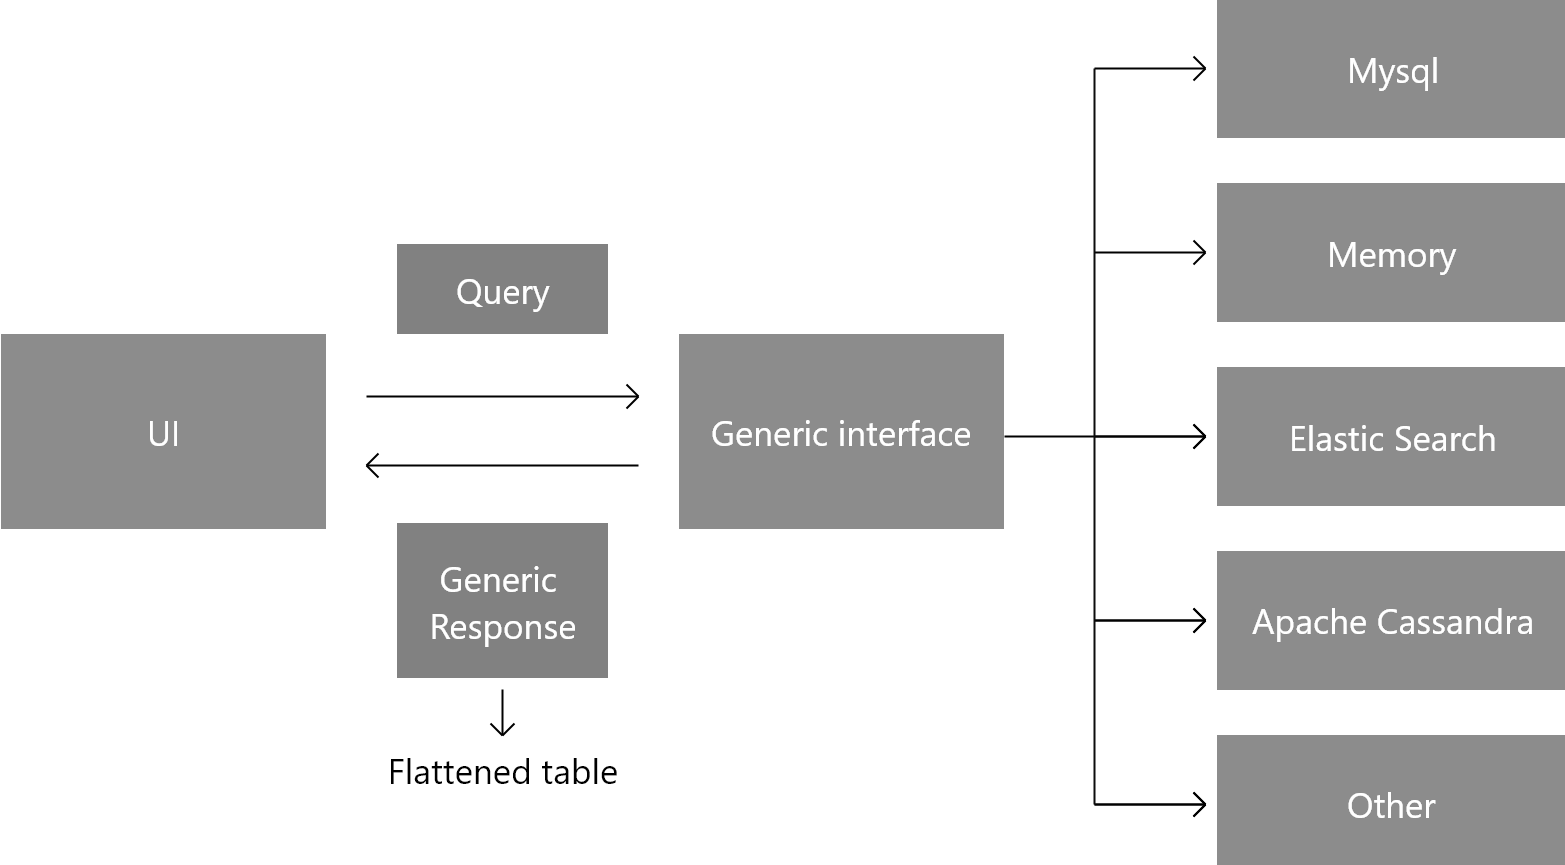
\includegraphics[scale=0.3]{generic-interface-flow.png}
        \caption{Scheme generic interface}
        \label{fig:generic-interface-flow}
    \end{figure}
\subsubsection{The flow of the generic interface}
    \begin{enumerate}
        \item{A user sends a request that contains a certain query. The query can be seen as a predefined structure comparable to an SQL query but with more capabilities to filter and on a higher level.}
        \item{Although I am not completely aware of the inner working, the generic interface maintains / collects data from different sources based on the provided query.}
        \item{The gathered data is filtered based on that same query.}
        \item{A response is sent back to the user in the shape of a \underline{flattened table}.}
    \end{enumerate}  
   
\section{flattened table}\label{generic-interface-flattened-table}

\subsection{Table}
Since the data is returned in a flat table it would be nice if this can be immediately visualized. A table is a rather simple but yet \textbf{very} powerful way to visualize information.

Due to the large amounts of data that Skyline's customers have to deal with, these tables often exist out of thousands of rows and dozens of columns. A table with these amounts of data quickly becomes inconvenient, obscure and generally not worth using. The main question took shape: 
\begin{center}
\textbf{How can we visualize large tabular data without sacrificing usability?}
\end{center}

** requires connection**
\begin{itemize}
    \item {Who are the users?}
    \item {What kind of functionalities do the users expect?}
    \item {What issues are they dealing with?}
    \item {Does Skyline solves certain issues already?}
    \item {Can the table be filtered to become easier to handle?}
\end{itemize}

\textbf{Note:} Although the focus is on Skyline Communications and the paper being completely written with Skyline in mind. The results will apply to other elaborations.

\textbf{The goal is should still be defined.}
